\input{header}
\physics
\begin{document}
\papertitle{Analysis of an Air Gyroscope's Precession}
\paperauth{A}{Khesin}{1002442029}
\paperauth{P}{Zavyalova}{1002345036}
\paperdate{March 28, 2018, Completed March 22, 2018}
\begin{paperabs}

	HEY SORRY FOR CAPS COULD YOU PLEASE TRY TO KEEP ``OBSERVATIONS'' RIGHT AT THE TOP OF PAGE TWO? THANKS
	
\end{paperabs}

\begin{paper}
	
\papersec{Introduction}
	
	The value of \textit{g} may be accurately determined by examining the precession of a gyroscopic rotator, an accurately machined sphere with a flat region. The sphere is driven by a coil to rotate with the axis of rotational symmetry horizontal. The rotator ends up being magnetized along an equatorial diameter and therefore together with the coil constitutes a synchronous motor. Since the rotor is free, the angular momentum vector may freely change its direction. 
	
	The change in the angular momentum vector of the rotor arises from a torque acting in the horizontal plane resulting from the imbalance from the truncated section of the sphere. A pure precession about a vertical axis arises due to the fact that the torque is at all times perpendicular to the angular momentum. 
	
	In this experiment, the above setup was implemented with the goal of approximating \textit{g}. Constant torsion-free air suspension supported the sphere. The rotor was accelerated using a controllable air flow until a frequency of \( 3600 \) rpm was attained. The frequency of rotation was measured using a strobe light; as soon as the desired value was obtained, the accelerating air flow was shut off and the driving coil was switched on. The rotator was driven at \( \pars{60 \pm .1} \si{\hertz} \) by a coil connected to the A.C. mains. To determine the period of rotation of the sphere, a laser light was reflected from the surface of the sphere. By marking the position of a well-defined spot resulting from specular reflection from the flat section and measuring the time of a full revolution, the period was obtained. The complete experimental setup is shown below.
	
	\paperfig{Setup}{\pdf{setup} \vspace{-2.5em}}{Experimental setup used for determining the value of \textit{g} through precession of an air gyroscope. The driving coil was mounted in the platform supporting the truncated sphere, a laser was aligned with the flat surface, and a strobe light was used to ensure that the desired frequency is maintained.}
	
	Expressions for torque \( L \) and moment of inertia of the rotator may be calculated by assuming a uniform density of the sphere. The dimensions of the gyroscopic rotator were denoted as follows.\\
	
	\paperfig{Sphere}{\hspace{4ex}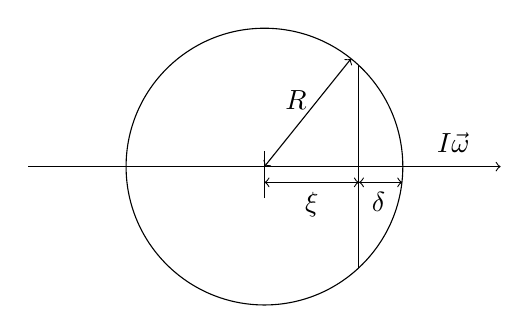
\begin{tikzpicture}
		\draw (0, 0) circle (50pt);
		\draw[->] (-3, 0)--(3, 0);
		\draw[-] (1.2, -1.29)--(1.2, 1.29);
		\draw[<->] (0, 0)--(1.1, 1.37);
		\draw[-] (0, -0.4)--(0, 0.2);
		\draw[<->] (0, -0.2)--(1.2, -0.2);
		\draw[<->] (1.2, -0.2)--(1.75, -0.2);
		\draw (0.6, -0.2) node[below] {\( \xi \)};
		\draw (1.45, -0.2) node[below] {\( \delta \)};
		\draw (0.4, 0.6) node[above] {\( R \)};
		\draw (2.4, 0.3) node {\( I\vec{\omega} \)};
	\end{tikzpicture}}{A sphere of radius \( R \) truncated to obtain a minimum distance from the center of \( R - \delta = \xi \), constituting a gyroscopic rotator. The angular momentum vector lies in the horizontal plane at all times and has a magnitude of \( I\omega \).}

\papersec{Observations}
	
Under the strobe light, the sphere came to a standstill, to the point where changing the strobe light frequency from 3600 flashes per minute by a few points would add noticable rotation to the sphere.
Thus, the frequency of the sphere's rotation was determined to be $(60\pm.02)\si{\hertz}$.
Additionally, this experiment does not work if the surface of rotation is not perfectly horizontal, the provided level was used to make sure that all areas of the surface were as level as possible.

The diameter of the sphere was measured with a capliper in several places, resulting in a value of $(50.525\pm.005)\si{\milli\meter}$ for the diameter, or $R=(25.263\pm.003)\si{\milli\meter}$ for the radius.
The ``diameter'' of the sphere measured along its axis of rotation was $(48.620\pm.005)\si{\milli\meter}$ resulting in a distance from the centre to the middle of the flat side of $\xi=(23.357\pm.006)\si{\milli\meter}$, meaning that the cutoff distance was measured to be $\delta=(1.905\pm.007)\si{\milli\meter}$.

The periods of revolution of the sphere obtained by marking a point on the wall and waiting for a steady laser to pass over the same point were recorded below.\\

\paperfig{T}{\begin{papertable}{|[outer]I|[inner]C|[outer]}\paperoline
\papertableindexheader&\textsc{Period}\\
\papertablecheadersymbol{T$ $(\pm\SI{1}{\second})}\\\paperiline
\papertableindex\papertablecval{635}\\\paperiline
\papertableindex\papertablecval{642}\\\paperiline
\papertableindex\papertablecval{645}\\\paperiline
\papertableindex\papertablecval{644}\\\paperiline
\papertableindex\papertablecval{645}\\\paperiline
\papertableindex\papertablecval{644}\\\paperiline
\papertableindex\papertablecval{645}\\\paperiline
\papertableindex\papertablecval{645}\\\paperiline
\papertableindex\papertablecval{646}\\\paperiline
\papertableindex\papertablecval{647}\\\paperoline
\end{papertable}\vspace{-1.5em}}
{The observed periods of rotation of the sphere. By discrading the first two measurements due to the fact that the sphere was still stabilising, yields an averarage period of $(645\pm1)\si{\second}$.}\\

The results in \figT show that the average rate of rotation of the sphere was one rotation every $(645\pm1)\si{\second}$.

\papersec{Analysis} 

First, a placeholder value called $\epsilon$ was calculated, which was the ratio between $\delta$ and $R$.

\papereq{E}{\epsilon=\frac\delta R}{gmg/gdl}
\begin{paperwhere}
\papervar{\epsilon}{fraction cut off}{}
\papervar{\delta}{distance cut off}{\meter}
\papervar{R}{radius of sphere}{\meter}
\end{paperwhere}

For the calculated values of $\delta$ and $R$, the value of $\epsilon$ was derived to be $(0.0754\pm.0003)$.
Next, the torque was calculated using the following formula, which is an expansion of the $r\cross F$ formula using the knowledge of the sphere's shape and simplified using the fact that $(r+a\cdot F)\cross F=r\cross F$.

\papereq{L}{\fontsize{9pt}{9pt}\selectfont\vec L=\rho g\int\limits_{\text-R}^{R-\delta}\int\limits_{\text-\sqrt{R^2-x^2}}^{\sqrt{R^2-x^2}}2\sqrt{R^2-x^2-y^2}(y,\text-x,0)\d y \d x}{}
\begin{paperwhere}
\papervar{\vec L}{torque}{\newton\metre}
\papervar{\rho}{density}{\kilo\gram\per\meter\cubed}
\papervar{g}{gravitational acceleration}{\meter\per\second\squared}
\end{paperwhere}

The resulting vector from \eqL is the vector (0,$(6.74\pm.02)\SI{E-9}{}\rho g$,0).
This is sensible as there is no torque in the $x$ or $z$ component, but only torque in the $y$ component.
Thus, $L=(3.37\pm.01)\SI{E-9}{}\rho g$.
Without plugging in the values of $R$ and $\delta$, the $y$ component of the above integrates to $\frac{\pi\delta^2(2r-\delta)^2\rho g}{4}$, which can be rewritten as $\frac{g\rho\pi R^4\epsilon^2(2-\epsilon)^2}{4}$.

For the moment of inertia of the sphere, the integral is done by subtracting the moment of intertia of the sliced off piece from that of a sphere, then integrating over expanding rings.
The result is the following.

\papereq{I}{\fontsize{9pt}{9pt}\selectfont I=\rho\left(\frac{8\pi R^5}{15}-\int\limits_{R-\delta}^{R}\int\limits_0^{\sqrt{R^2-x^2}}2\pi r^3\d r\d x\right)}{}
\begin{paperwhere}
\papervar{I}{moment of inertia}{\meter\square\kilo\gram}
\end{paperwhere}

The result from \eqI is $I=(1.72\pm.01)\SI{E-8}{}\rho$.
Without plugging in the values of $R$ and $\delta$, the above integrates to $\rho\left(\frac{8\pi R^5}{15}-\frac{\delta^3\pi(3\delta^2-15\delta R+20R^2)}{30}\right)$, which can be rewritten as $\frac{\rho\pi R^5(2-\epsilon)^3(\epsilon^2+\epsilon+\frac23)}{10}$.

It is known that the ratio of the torque and the product of the moment of inertia and the angular velocity about the sphere's axis is equal to the angular velocity of the precession in the plane.
But the angular velocities are given by the ratio of $2\pi$ by the period, thus we get the following.

\papereq{R}{\frac{2\pi}{T}\cdot\frac{2\pi}{\frac{1}{60}}=\frac{L}{I}}{}
\begin{paperwhere}
\papervar{T}{precession period}{\second}
\end{paperwhere}

Note that by taking the ratios of \eqL and \eqI, we can derive an expression equivalent to \eqR.

\papereq{S}{\frac LI=\frac{5g\epsilon^2}{2R(2-\epsilon)(\epsilon^2+\epsilon+\frac23)}}{}

By plugging in all the obtained values, and equating \eqR and \eqS, we get that
$(3.67\pm0.08)\si{\per\second\squared}=(0.39\pm.02)\si{\per\metre}g$.
Thus, we obtain the final result of $g=(9.79\pm.02)\si{\metre\per\second\squared}$.

\papersec{Conclusion}

	Conclusion goes here
	
\papersec{Sources}

	\papersource{`g' Using Precession of an Air Gyroscope, gmg/gdl -- 1971, jbv 1990}

\end{paper}
\end{document}